\originalchapter{进阶作业五：相互作用与量子系综}
\psource{8.333，2013 秋，Problem Set 5，11 月 22 日截止；全 12 题，原选做 3、5、7、11 也纳入。官方未公开本卷答案；本章全部为 AI 独立解答，经独立复核，并非 MIT 官方答案。}
\originalsection{1．表面活性剂凝聚}
\begin{exercise}
水面面积 $A$ 上 $N$ 分子二维位置、动量 $\vct q_i,\vct p_i$，$H=\sum p_i^2/(2m)+\sum_{i<j}V(\vct q_i-\vct q_j)$。忽略与水本身耦合；$V(r)=\infty$（$r<a$），$r>a$ 吸引满足 $\int_a^\infty2\pi rV(r)\dd r=-u_0$。
(a) 写相空间正则 $Z$ 并积分动量；(b) 估计非排除的位置相空间；(c) 均匀密度 $n=N/A$ 估势能并给近似 $Z$；(d) 清水张力 $\sigma_0$ 基本不随温度变，求加入分子后的张力；(e) 找温度以下模型明显失效并解释低温行为；(f) 求 $C_A$，给不要求显算的 $C_\sigma$ 表达式。
\end{exercise}
\begin{solution}
(a) $Z=(N!h^{2N})^{-1}\int\dd^{2N}p\dd^{2N}q\,e^{-\beta H}= (N!\lambda_T^{2N})^{-1}\int\dd^{2N}q\,e^{-\beta\sum V}$。
(b) 依次放置的粗略体积 $\prod_{j=0}^{N-1}(A-j\pi a^2)$；低密度对数展开的领先项可用 $(A-Nb)^N$ 匹配，$b=\pi a^2/2$。这一范德瓦耳斯重求和在高密度仅是模型，不能当作精确几何。
(c) 每分子势平均 $-nu_0$，双计数除二，$U_{\rm att}\simeq-u_0N^2/(2A)$；因此 $Z\simeq(A-Nb)^N e^{\beta u_0N^2/(2A)}/(N!\lambda_T^{2N})$。
(d) 分子铺展压 $\Pi=\kb Tn/(1-bn)-u_0n^2/2$，总张力 $\sigma=\sigma_0-\Pi$。
(e) 稳定膜要求 $\Pi_n\ge0$；$\Pi_n=\kb T/(1-bn)^2-u_0n$。其最小允许温度在 $n_c=1/(3b)$，$\kb T_c=4u_0/(27b)$。$T<T_c$ 一段密度有负压缩稳定性，应分为稀密两表面相；均场不能正确预测全部相分离细节。
(f) $U=N\kb T-u_0N^2/(2A)$，所以 $C_A=N\kb$。在稳定单相 $C_\sigma=C_A+T\sigma_T^2/\sigma_A$（固定 $N$）；因 $\dd F=-S\dd T+\sigma\dd A$，$S_A=-\sigma_T$、$A_T|_\sigma=-\sigma_T/\sigma_A$。清水常张力无此项，且其未知热容未计入。
\end{solution}
\originalsection{2．三阶状态方程的临界点}
\begin{exercise}
$P=\kb Tn-bn^2/2+cn^3/6$，$b,c>0$ 恒定。
(a) 求失稳临界 $T_c,n_c,P_c$ 及 $\kb T_cn_c/P_c$；(b) 求 $\kappa_T$，画 $n=n_c$ 时随 $T$ 变化；(c) 临界等温线上 $P-P_c$ 与 $n-n_c$ 的关系；(d) $T<T_c$ 两相密度近似 $n_\pm\simeq n_c(1\pm\delta)$，用 Maxwell 或 $\dd\mu=\dd P/n$ 给 $\delta(T)$ 隐式关系及 $T\uparrow T_c$ 行为。
\end{exercise}
\begin{solution}
(a) $P_n=P_{nn}=0$ 给 $n_c=b/c$、$\kb T_c=b^2/(2c)$、$P_c=b^3/(6c^2)$，比值 3。
(b) $\kappa_T=[n(\kb T-bn+cn^2/2)]^{-1}$；在 $n_c$ 为 $1/[n_c\kb(T-T_c)]$，上方正且发散，下方负表示模型均匀相不稳定。
(c) 正好 $P-P_c=c(n-n_c)^3/6$，平均场临界指数 3。
(d) 精确共存隐式方程为 $P(n_+)=P(n_-)$ 与
\[\kb T\ln(n_+/n_-)-b(n_+-n_-)+\frac c4(n_+^2-n_-^2)=0.\]
将题给对称\textbf{领先}近似代第二式，$T/T_c\simeq2\delta/\ln[(1+\delta)/(1-\delta)]$。小 $\delta$ 展开给 $\delta^2\simeq3(1-T/T_c)$，即指数 $1/2$。第一式在此近似同样给 $T/T_c\simeq1-\delta^2/3$。二式在更高阶不能同时以严格对称密度满足，应保留中心密度的 $O(\delta^2)$ 位移并解精确双方程；不把领先对称关系冒作全温精确 binodal。
\end{solution}
\begin{center}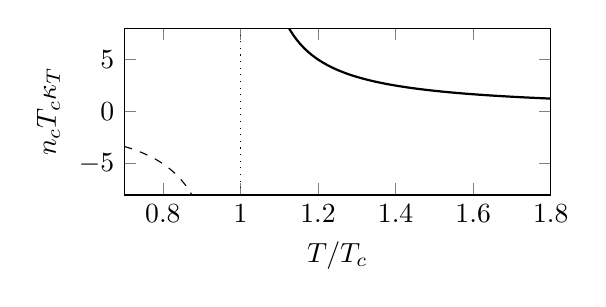
\begin{tikzpicture}\begin{axis}[width=7cm,height=3.7cm,xmin=.7,xmax=1.8,ymin=-8,ymax=8,xlabel={$T/T_c$},ylabel={$n_c\kb T_c\kappa_T$},samples=80]\addplot[domain=.7:.96,dashed]{1/(x-1)};\addplot[domain=1.04:1.8,thick]{1/(x-1)};\draw[dotted](axis cs:1,-8)--(axis cs:1,8);\end{axis}\end{tikzpicture}\end{center}
\originalsection{3．Manning 转变（原选做）}
\begin{exercise}
忽略离子互斥，长 $L$、半径 $a$ 的带电柱在半径 $R$ 容器中，$N$ 个反离子，$n=N/L$，经典
\[H=\sum_i[p_i^2/(2m)+2e^2n\ln(r_i/R)],\qquad a\le r_i\le R.\]
(a) 求 $Z(T,n,R,a)$；(b) 求径向密度与平均半径；(c) $R\gg a$ 确定转变温度、两相及平均半径依赖；(d) 全温求大容器侧壁压力；(e) 考虑互斥的粗模型让 $N_1$ 凝在柱旁、$N_2=N-N_1$ 自由，自由离子势把 $n$ 换成 $n_2=N_2/L$；猜平衡 $N_2^*$，以微小偏离的响应定性论证，无须新计算。
\end{exercise}
\begin{solution}
设 $\xi=\beta e^2n$、$s=2-2\xi$、$t=a/R$，并记 $J_s=\int_a^Rr^{s-1}\dd r=(R^s-a^s)/s$，$s=0$ 时为 $\ln(R/a)$。
(a) $z=(2\pi L/\lambda_T^3)R^{2\xi}J_s$，$Z=z^N/N!$。
(b) $p(r)=r^{s-1}/J_s$，$\avg r=J_{s+1}/J_s$；$s=-1$ 时分子为对数，其他退化点取连续极限。
(c) 临界 $\xi=1$，$\kb T_c=e^2n$。$\xi<1$ 时 $\avg r\sim R(2-2\xi)/(3-2\xi)$，离子向容器扩散。$\xi=1$ 时 $\avg r\sim R/\ln(R/a)$。$1<\xi<3/2$ 时 $\avg r\sim[(2\xi-2)/(3-2\xi)]a^{2\xi-2}R^{3-2\xi}$，虽径向概率集中近柱，稀尾仍使均值发散；$\xi=3/2$ 时 $\avg r\sim a\ln(R/a)$，$\xi>3/2$ 时 $\avg r\sim a(2\xi-2)/(2\xi-3)$。因此“低温凝聚”不等于所有低温平均半径都有限。
(d) 物理接触压力是侧壁局部 $P_w=\kb T\,N R^{-2\xi}/(2\pi L J_s)$，所以 $R\gg a$ 时，$\xi<1$：$P_w\sim n\kb T(1-\xi)/(\pi R^2)$；$\xi=1$：$n\kb T/[2\pi R^2\ln(R/a)]$；$\xi>1$：$n\kb T(\xi-1)a^{2\xi-2}/(\pi R^{2\xi})$。题势零点随 $R$ 移动，直接对含 $R$ 的 $Z$ 求导会额外计入基准移动，应先恢复固定基准（把 $R$ 改固定参考长度）再用热力学导数；结果与接触定理相同。
(e) 若 $T\ge T_c$，$N_2^*=N$；若 $T<T_c$，自由线密度自调至 $n_2^*=\kb T/e^2$，$N_2^*=L\kb T/e^2$，凝聚比例 $1-T/T_c$。自由数稍过多则 $\xi_2>1$，吸引促进一步凝聚；稍少则 $\xi_2<1$，热扩散促释放。此为近似反馈论证，不代替完整相关离子理论。
\end{solution}
\originalsection{4．点粒子的所谓凝聚}
\begin{exercise}
三维经典点粒子 $Z=Z_{\rm ideal}\exp[\beta uN^2/(2V)]$，$u>0$。
(a) 全部能量累积量 $\avg{H^p}_c$；(b) $P(n,T)$；(c) $\kappa_T$；(d) “凝聚线” $P_c(T)$。
\end{exercise}
\begin{solution}
$\ln Z=\mathrm{const}-(3N/2)\ln\beta+\beta uN^2/(2V)$。
(a) 第一累积量 $3N/(2\beta)-uN^2/(2V)$；$p\ge2$ 时 $\kappa_p=(3N/2)(p-1)!\beta^{-p}$，常能量平移不改高阶累积量。
(b) $P=n\kb T-un^2/2$。
(c) $\kappa_T=[n(\kb T-un)]^{-1}$。
(d) 局部均匀相失稳点 $n_c=\kb T/u$、$P_c=(\kb T)^2/(2u)$，这是 spinodal 最大压曲线。此模型无排斥，$V\to0$ 自由能无下界，不存在有限密度稳定液相，也没有可由等自由能求出的真实平衡凝聚线；若沿用题名，必须标明它仅指塌缩失稳界。
\end{solution}
\originalsection{5．二维硬杆（原选做）}
\begin{exercise}
二维长度 $2l$ 的杆可平移和绕中心转动，硬芯近似为每杆可转角 $\theta\in[0,\pi]$ 与相应排除面积 $\Omega(\theta)$，旋转相空间 $\mathcal A(\theta)$。固定面积 $V$、密度 $n=N/V$，忽略动量，大 $N$ 最大熵定角。
(a) 写 $S(N,n,\Omega,\mathcal A)$；(b) 驻值条件给 $n=f(\Omega,\mathcal A,\Omega',\mathcal A')$；(c) 根据原图的转动杆扫过区域外包形状求 $\Omega$，取 $\mathcal A\propto\theta$ 画 $f$；(d) 描述高密度状态、随密度下降的转变，标临界密度、给临界角隐式关系，无须显解；$n<n_c$ 时角为何？
\end{exercise}
\begin{solution}
(a) 原图单杆近似有效位置体积 $(V-N\Omega)^N/N!$，故 $S=N\kb\{\ln[(1/n-\Omega)\mathcal A]+1\}+\text{态单元常数}$，需 $n\Omega<1$。
(b) 对 $\theta$ 求导，$-n\Omega'/(1-n\Omega)+\mathcal A'/\mathcal A=0$，所以 $n=\mathcal A'/(\mathcal A\Omega'+\mathcal A'\Omega)$。
(c) 原图杆端距中心 $l$。两端扫过圆弧，外包的中央矩形面积 $2l^2\sin\theta$，两圆弓总面积 $l^2(\theta-\sin\theta)$，故 $\Omega=l^2(\theta+\sin\theta)$。这是原图的单杆\textbf{几何近似}，不是严格两杆 Mayer 排除面积。取 $\mathcal A=C\theta$，
\[f(\theta)=\frac1{l^2[2\theta+\sin\theta+\theta\cos\theta]}.\]
从 $\theta=0$ 的无穷降至极小再回升到 $1/(\pi l^2)$。驻值曲线折点满足 $2+2\cos\theta-\theta\sin\theta=0$，它是内点极大熵解出现的界，不能自动等同全局转变。
(d) 高密度小角有序，$\theta\simeq1/(4nl^2)$。低密度全转动端点 $\theta=\pi$ 的熵较大。全局转变须比较两种可达熵，临界内点 $\theta_c$ 满足
\[n_c=f(\theta_c),\qquad
\theta_c[1-n_c l^2(\theta_c+\sin\theta_c)]=\pi[1-n_c\pi l^2].\]
等价令 $f(\theta_c)=(\pi-\theta_c)/[l^2(\pi^2-\theta_c^2-\theta_c\sin\theta_c)]$，取非端点、内极大且 $n_c<1/(\pi l^2)$ 的根。角从内点跳至 $\pi$，为此粗模型的一阶转变；$n<n_c$ 取 $\pi$。最小 $f$ 只给亚稳解的极限。数值为 $\theta_c=1.199177921$、$n_cl^2=0.265565680$；驻值折点 $\theta_f=1.720667178$、$n_fl^2=0.239623628$。附录实算作图验证此模型的熵比较，不是严格硬杆相变证明。
\end{solution}
\begin{center}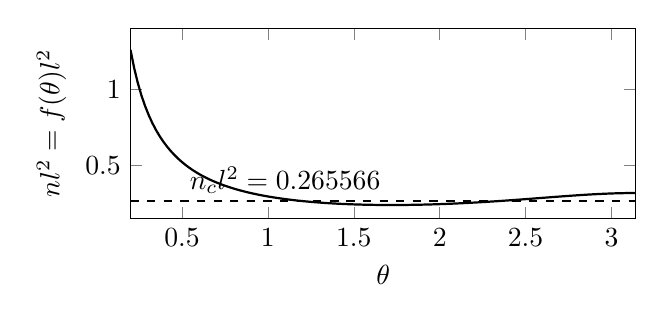
\begin{tikzpicture}\begin{axis}[width=8cm,height=4cm,xmin=.2,xmax=3.142,ymin=.15,ymax=1.4,xlabel={$\theta$},ylabel={$nl^2=f(\theta)l^2$},samples=140]\addplot[domain=.2:3.14159,thick]{1/(2*x+sin(deg(x))+x*cos(deg(x)))};\addplot[domain=.2:3.14159,dashed]{.265565680};\node at(axis cs:1.1,.4){$n_c l^2=0.265566$};\end{axis}\end{tikzpicture}\end{center}
\originalsection{6．电子自旋密度矩阵}
\begin{exercise}
$H=-\mu_B\vct\sigma\cdot\vct B$，$\mu_B$ 为 Bohr 磁子，Pauli 矩阵 $\sigma_x=\left(\begin{smallmatrix}0&1\\1&0\end{smallmatrix}\right)$、$\sigma_y=\left(\begin{smallmatrix}0&-i\\i&0\end{smallmatrix}\right)$、$\sigma_z=\left(\begin{smallmatrix}1&0\\0&-1\end{smallmatrix}\right)$。
(a) 场沿 $z$ 求正则 $\rho$；(b) 场沿 $x$ 重复；(c) 两情形平均能量。
\end{exercise}
\begin{solution}
令 $x=\beta\mu_BB$。由 $\sigma_j^2=1$，$e^{x\sigma_j}=\cosh x+\sigma_j\sinh x$。
(a) $\rho_z=\mathrm{diag}(e^x,e^{-x})/(2\cosh x)$。
(b) 在同一 $\sigma_z$ 基中 $\rho_x=\tfrac12\left(\begin{smallmatrix}1&\tanh x\\\tanh x&1\end{smallmatrix}\right)$，非对角元不能略去。
(c) 两者 $U=-\mu_BB\tanh x$；旋转场方向不改能谱，自由能相同。
\end{solution}
\originalsection{7．平面量子转子（原选做）}
\begin{exercise}
$H=-\hbar^2\partial_\theta^2/(2I)$，$0\le\theta<2\pi$，周期波函数。
(a) 本征态与能级；(b) 温度 $T$ 的 $\bra{\theta'}\rho\ket\theta$，评价低温、高温极限。
\end{exercise}
\begin{solution}
(a) $\psi_m=e^{im\theta}/\sqrt{2\pi}$，$m\in\mathbb Z$，$E_m=\epsilon_Rm^2$，$\epsilon_R=\hbar^2/(2I)$。
(b) $\rho(\theta',\theta)=(2\pi Z)^{-1}\sum_m e^{-\beta\epsilon_Rm^2}e^{im(\theta'-\theta)}$，$Z=\sum_m e^{-\beta\epsilon_Rm^2}$。低温基态独占，核趋 $1/(2\pi)$（纯态投影）。高温 Poisson 求和给
\[\rho(\theta',\theta)\simeq\frac1{2\pi}\sum_{j\in\mathbb Z}\exp\left[-\frac{I(\theta'-\theta+2\pi j)^2}{2\beta\hbar^2}\right],\]
$Z\simeq\sqrt{2\pi I/(\beta\hbar^2)}$，非对角相干宽度 $\sqrt{\beta\hbar^2/I}$，对角恒为 $1/(2\pi)$。不能把无限维高温 $\rho$ 写作“恒等算符除无穷”而当成正规密度矩阵。
\end{solution}
\originalsection{8．量子熵最大化}
\begin{exercise}
$S=-\Tr(\rho\ln\rho)$，本题熵未乘 $\kb$。
(a) 写 $\rho(t)$ 演化方程并求 $\dd S/\dd t$；(b) 归一化且固定 $\Tr\rho H=E$，用乘子求最大熵密度算符；(c) 证明所得解静止。
\end{exercise}
\begin{solution}
(a) 封闭系统 $i\hbar\dot\rho=[H,\rho]$，幺正共轭保全部本征值，故熵恒定。形式上 $\dot S=-\Tr[\dot\rho(\ln\rho+1)]=0$，零本征值用连续极限定义。
(b) 变分 $S-\alpha(\Tr\rho-1)-\beta(\Tr\rho H-E)$，得 $\ln\rho+1+\alpha+\beta H=0$，所以 $\rho_{\max}=e^{-\beta H}/Z$，$Z=\Tr e^{-\beta H}$，$\beta$ 由给定能量确定。最大性由量子相对熵非负证明：同能量时 $S(\rho_{\max})-S(\rho)=D(\rho\Vert\rho_{\max})\ge0$；须 $Z$ 有限、约束可实现。
(c) $\rho_{\max}$ 是 $H$ 的函数，与之对易，$\dot\rho=0$。开放系统熵可变化，不能将 (a) 外推到与热库耦合的演化。
\end{solution}
\originalsection{9．零点能的渐近匹配}
\begin{exercise}
经典谐振子 $H=p^2/(2m)+m\omega^2q^2/2$；假设量子谱 $E_n=x+yn$，$n\ge0$。
(a) 以 $\dd p\dd q/h$ 求 $Z_{\rm cl},E_{\rm cl}$；(b) 求 $Z_{\rm qm}$，高温匹配确定 $y$；(c) 求量子能，$\beta\to0$ 展开前两项，通过与经典匹配确定 $x$。
\end{exercise}
\begin{solution}
(a) $Z_{\rm cl}=2\pi/(\beta h\omega)=1/(\beta\hbar\omega)$，$E_{\rm cl}=1/\beta$。
(b) $Z_{\rm qm}=e^{-\beta x}/(1-e^{-\beta y})\sim1/(\beta y)$，所以 $y=\hbar\omega$。
(c) $E_{\rm qm}=x+y/(e^{\beta y}-1)=1/\beta+(x-y/2)+\beta y^2/12+O(\beta^3)$。要求\textbf{常数项也与给定经典能量零点一致}，则 $x=y/2=\hbar\omega/2$。仅要求高温相对误差趋零不足以确定任何有限 $x$；题目实际采用更强的渐近匹配及相同势零点。零点能的完整物理依据仍是量子振子的本征问题。
\end{solution}
\originalsection{10．高温量子热容修正}
\begin{exercise}
(a) 量子谐振子求 $Z_{\rm vib}$ 并将 $\ln Z$ 展开到 $(\beta\hbar\omega)^2$；(b) 求量子化对振动高温热容的第一修正。
给 Abel--Plana 公式 $\sum_{n=0}^\infty f(n)=\int_0^\infty f(x)\dd x+f(0)/2+i\int_0^\infty[f(it)-f(-it)]/(e^{2\pi t}-1)\dd t$。
(c) 用它核对小 $u$ 的几何和 $\sum e^{-nu}$；(d) 用该方法说明 $\sum_{\ell\ge0}(2\ell+1)e^{-u\ell(\ell+1)}=1/u+1/3+u/15+O(u^2)$；(e) 求三维转子高温能量，惯量 $I$；(f) 转动热容的第一量子修正。
\end{exercise}
\begin{solution}
(a) 令 $x=\beta\hbar\omega$，$Z=e^{-x/2}/(1-e^{-x})=[2\sinh(x/2)]^{-1}$，$\ln Z=-\ln x-x^2/24+O(x^4)$。
(b) $C=\kb[1-x^2/12+O(x^4)]$。
(c) $f(z)=e^{-uz}$ 的主积分 $1/u$，边界 $1/2$，第三项 $2\int\sin(ut)/(e^{2\pi t}-1)\dd t$。用 $J_j=\int_0^\infty t^j/(e^{2\pi t}-1)\dd t=\Gamma(j+1)\zeta(j+1)/(2\pi)^{j+1}$，$J_1=1/24,J_3=1/240$，得 $1/u+1/2+u/12-u^3/720+\cdots$，与 $1/(1-e^{-u})$ 相同。
(d) $f(z)=(2z+1)e^{-uz(z+1)}$ 的实轴积分恰 $1/u$，$f(0)/2=1/2$。形式第三项分子为 $2e^{ut^2}[\sin(ut)-2t\cos(ut)]$；展开至一阶为 $-4t+u(2t-4t^3)$，积分系数给 $-4J_1=-1/6$、$2J_1-4J_3=1/15$，得所求。
此处必须说明\textbf{所给 Abel--Plana 无穷积分不可对该 $f$ 直接使用}：虚轴的 $e^{ut^2}$ 使积分发散。上述是渐近系数计算，严格余项可由有限轮廓版本或 Euler--Maclaurin 得到。为补齐合法论证，Euler--Maclaurin 的端点修正为 $-f'(0)/12+f'''(0)/720-\cdots$；$f'(0)=2-u$、$f'''(0)=-12u+O(u^2)$，因此 $1/2-(2-u)/12-12u/720=1/3+u/15$，将 Euler--Maclaurin 保留到 $B_6f^{(5)}(0)/6!$，$f^{(5)}(0)=O(u^2)$，其余项满足
\[|R_3|\le\frac{2\zeta(6)}{(2\pi)^6}\int_0^\infty|f^{(6)}(x)|\dd x.\]
设 $y=\sqrt u(x+1/2)$，$f=2e^{u/4}u^{-1/2}y e^{-y^2}$，积分为 $2e^{u/4}u^2\int_{\sqrt u/2}^\infty|\partial_y^6(ye^{-y^2})|\dd y=O(u^2)$，故所求余项有界。对参数导数同样应用该展开，可得余项一、二导数分别 $O(u),O(1)$，为下述能量与热容展开的逐次求导提供控制。附录的直接谱和仅数值验证渐近误差，不当作余项证明。
(e) $\epsilon_R=\hbar^2/(2I)$、$u=\beta\epsilon_R$，$\ln Z=-\ln u+u/3+u^2/90+O(u^3)$，所以 $U=\kb T-\epsilon_R/3-\epsilon_R^2/(45\kb T)+\cdots$。
(f) $C_R=\kb[1+\epsilon_R^2/(45(\kb T)^2)+O(u^3)]$；振动修正为负而转动此阶为正。
\end{solution}
\originalsection{11．平衡正氢与仲氢（原选做）}
\begin{exercise}
氢分子核质子对，仲氢为反对称单态，转动 $\ell=0,2,4,\ldots$；正氢为对称三重态，转动 $\ell=1,3,5,\ldots$，能量均 $\hbar^2\ell(\ell+1)/(2I)$。
(a)(b) 各转动配分函数与低/高温极限；(c) 求 $N$ 分子\textbf{平衡}气体配分函数，忽略振动，可对 $N_p,N_o=N-N_p$ 求和；(d) 旋转内能表达式与两端极限。现实转化速率小，混合物常未达到正仲平衡。
\end{exercise}
\begin{solution}
令 $u=\beta\epsilon_R$，
\[z_p=\sum_{\ell\text{偶}}(2\ell+1)e^{-u\ell(\ell+1)},\quad
z_o=3\sum_{\ell\text{奇}}(2\ell+1)e^{-u\ell(\ell+1)}.\]
低温 $z_p=1+5e^{-6u}+\cdots$、$z_o=9e^{-2u}+21e^{-12u}+\cdots$；高温 $z_p\sim1/(2u)$、$z_o\sim3/(2u)$，核自旋三重因子不得遗漏。
(c) 经典平动单态 $z_t=V/\lambda_T^3$，各组成 $Z_{N_p,N_o}=z_t^Nz_p^{N_p}z_o^{N_o}/(N_p!N_o!)$；求和 $Z=z_t^N(z_p+z_o)^N/N!$。
(d) $U_R=-N\partial_\beta\ln(z_p+z_o)$。低温主要从全仲基态激发到 $\ell=1$，$U_R\simeq18N\epsilon_Re^{-2u}$；高温 $U_R\simeq N\kb T$。固定组成未平衡时应用 $U_R=-N_p\partial_\beta\ln z_p-N_o\partial_\beta\ln z_o$，低温可仍有正氢 $2\epsilon_RN_o$ 的能量，不能套平衡结果。
\end{solution}
\originalsection{12．经典 van Leeuwen 定理}
\begin{exercise}
$N$ 个带电粒子 $H=\sum_i p_i^2/(2m)+U(\vct q_1,\ldots,\vct q_N)$。外磁场下规范动量换为 $\vct p_i-e\vct A(\vct q_i)$，$\vct B=\nabla\times\vct A$。证明忽略量子效应时热力学与 $B$ 无关。
\end{exercise}
\begin{solution}
经典正则积分在每个固定位置进行全 $\mathbb R^3$ 动量积分，平移 $\vct\pi_i=\vct p_i-e\vct A(\vct q_i)$，Jacobian 为一、积分域不变，
\[Z=\frac{(2\pi m/\beta)^{3N/2}}{N!h^{3N}}\int\dd^{3N}q\,e^{-\beta U(q)},\]
所以 $F=-\kb T\ln Z$ 无 $B$，轨道磁化为零。位置--动量整体变换虽未必规范，这里只用积分变元代换，不需它规范。条件是 $U$ 不另含磁性、自旋等场项，平衡动量无人工截断；实际磁性来自量子效应或超出此题的自由度。时间轨道可受 Lorentz 力改变而平衡自由能仍不变。
\end{solution}
